%(BEGIN_QUESTION)
% Copyright 2010, Tony R. Kuphaldt, released under the Creative Commons Attribution License (v 1.0)
% This means you may do almost anything with this work of mine, so long as you give me proper credit

Examine this chromatogram showing two peaks, and determine which peak represents the greatest quantity of substance:

$$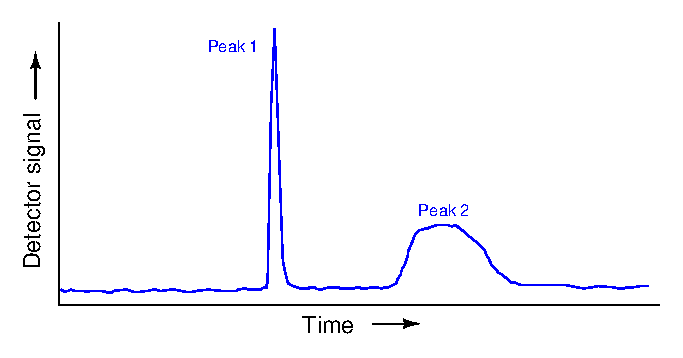
\includegraphics[width=15.5cm]{i04156x01.eps}$$

Explain {\it why} you interpreted the peaks as you did.

\vskip 10pt

Now suppose the concentration of substance causing peak 1 suddenly increases in the sample stream, while the concentration of the other substance does not change.  How would this change in the sample's composition affect the appearance of subsequent chromatograms?

\vskip 20pt \vbox{\hrule \hbox{\strut \vrule{} {\bf Suggestions for Socratic discussion} \vrule} \hrule}

\begin{itemize}
\item{} Explain how the calculus concept of {\it integration} applies to this question.
\item{} Suppose you were informed this chromatogram was taken off the detector's raw signal, unscaled by any {\it response factors}.  Would your interpretation of the chromatogram be any different with this knowledge?
\end{itemize}

\underbar{file i04156}
%(END_QUESTION)





%(BEGIN_ANSWER)


%(END_ANSWER)





%(BEGIN_NOTES)

Assuming that proper response factors have been programmed into this chromatograph to proportionately scale each peak according to molecular quantity, peak 2 on the chromatogram represents the larger molecular quantity, because the {\it area} enclosed by the peak is greater.  Peak 1, despite being taller, encloses less area, and therefore represents a smaller molecular quantity.

If the substance represented by peak 1 were to increase, peak 1 would grow in area without affecting its timing or the area/timing of peak 2 (assuming the concentration of substance represented by peak 2 did not change).

\vskip 10pt

A common misconception of students learning chromatography is to assume the {\it timing} of chromatogram peaks is related to substance concentration, when in fact only the peak area is affected by changes in concentration.









\vfil \eject

\noindent
{\bf Summary Quiz}

Examine this chromatogram and identify the {\it two} best statements describing this analysis:

$$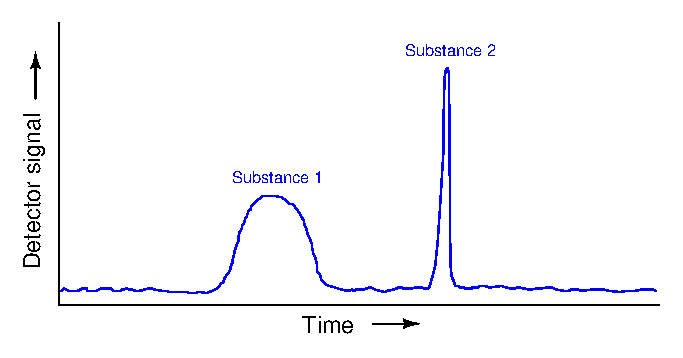
\includegraphics[width=15.5cm]{i04156x02.eps}$$

\begin{itemize}
\item{} There is more of substance 1 than of substance 2 in the sample.
\vskip 5pt
\item{} Substance 1 was injected into the column before substance 2.
\vskip 5pt
\item{} Substance 1 has the least retention time.
\vskip 5pt
\item{} There is more of substance 2 than of substance 1 in the sample.
\vskip 5pt
\item{} Both substances (peak 1 and 2) have the same retention time.
\vskip 5pt
\item{} Substance 2 was injected into the column before substance 1. 
\vskip 5pt
\item{} Substance 2 has the least retention time.
\vskip 5pt
\item{} There are equal quantities of substance 1 and 2 in the sample.
\end{itemize}


%INDEX% Measurement, analytical: chromatography

%(END_NOTES)


